\documentclass[../main.tex]{subfiles}
\graphicspath{{\subfix{../images/}}}
\begin{document}
\section*{Term 2 Week 2}
\begin{enumerate}
    \item 
    The right-angled triangle ABC has sides AB = 3 cm, AC = 5 cm and BC = 4 cm.\\
    
    Three arcs are drawn with centres at each of the vertices so that each of them touches the other two.\\
    
    Find the size of the shaded area enclosed by the three arcs.\\
    \begin{figure}[h]
        \centering
        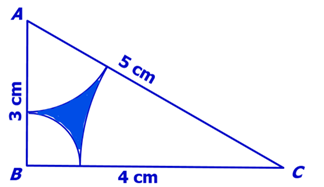
\includegraphics{images/t2w2q1.png}
    \end{figure}

    \item 
    A solid metal sphere is completely immersed in acid and dissolves at a rate directly proportional to its surface area. After \textit{m} minutes, the volume is reduced by a half. How long, in terms of \textit{m}, does it take to completely dissolve the sphere?\\

    \item 
    If \(f(n)=3^{n+1}+2^n\), find \textit{a} and \textit{b} such that \(f(n+2)=a.f(n+1)+b.f(n)\)\\

    \item 
    Evaluate:\\
    \[\sum_{k=1}^\infty \frac{1}{4k^2-1}\]\\

    \item 
    Three circles are drawn sitting on a straight line so that they are tangential to each other and to the line (see diagram below). Given that the radius of the largest circle is \textit{a}, the radius of the medium circle is \textit{b}, and the smallest radius is \textit{r}, prove that \(\frac{1}{\sqrt{r}}=\frac{1}{\sqrt{a}}+\frac{1}{\sqrt{b}}\)\\
    \begin{figure}[H]
        \centering
        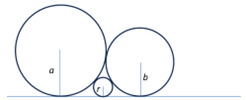
\includegraphics{images/t2w2q5.png}
    \end{figure}
    
    
\end{enumerate}

\end{document}